\section*{Phần 1.2}
\subsection*{Bài 6}
Bạn chỉ có thể nâng cấp hệ điều hành khi bạn có một vi xử lí 32-bit có xung clock từ 1 GHz, ít nhất 1 GB RAM, và 16 GB dung lượng còn dư, hoặc một vi xử lí 64-bit có xung clock từ 2 GHz, ít nhất 2 GB RAM, và ít nhất 32 GB dung lượng còn dư. Thể hiện câu trả lời thông qua $u$: "Bạn có thể nâng cấp hệ điều hành", $b_{32}$: "Bạn có một vi xử lí 32-bit", $b_{64}$: "Bạn có một vi xử lí 64-bit", $g_1$: "Vi xử lí của bạn có xung clock là 1 GHz hoặc cao hơn", $g_2$: "Vi xử lí của bạn có xung clock là 2 GHz hoặc cao hơn", $r_1$: "Vi xử lí của bạn có ít nhất 1 GB RAM",  $r_2$: "Vi xử lí của bạn có ít nhất 2 GB RAM", $h_{16}$: "Bạn có ít nhất 16 GB dung lượng trống", $h_{32}$: "Bạn có ít nhất 32 GB dung lượng trống".
\begin{proof}
    Ta viết lại câu hỏi: \textbf{Nếu} bạn có một vi xử lí 32-bit từ 1 GHz, \textbf{và} ít nhất 1 GB RAM, \textbf{và} 16 GB dung lượng còn dư, \textbf{hoặc} một vi xử lí 64-bit từ 2 GHz, \textbf{và} ít nhất 2 GB RAM, \textbf{và} ít nhất 32 GB dung lượng còn dư, \textbf{thì} bạn có thể nâng cấp hệ điều hành. Vậy đáp án là: $$(b_{32}\land g_1\land r_1\land h_{16})\lor(b_64\land g_2\land r_2\land h_{32})\rightarrow u$$
\end{proof}
\subsection*{Bài 7}
Thể hiện các yêu cầu hệ thống sau đây dùng mệnh đề $p$: "Tin nhắn đã được quét virus" và $q$: "Tin nhắn được gửi từ một hệ thống lạ", dùng các kí hiệu logic (kể cả phép phủ định).
\begin{enumerate}[label=\alph*)]
    \item "Tin nhắn đã được quét virus mỗi khi tin nhắn được gửi từ một hệ thống lạ"
    \item "Tin nhắn được gửi từ một hệ thống lạ nhưng tin nhắn chưa được quét virus"
    \item "Mỗi khi tin nhắn được gửi từ một hệ thống lạ, quét virus tin nhắn là điều cần thiết"
    \item "Khi tin nhắn được gửi từ một hệ thống đã biết thì tin nhắn không được quét virus"
\end{enumerate}
\begin{proof}.
    \begin{multicols}{4}
        \begin{enumerate}[label=\alph*)]
            \item $p\leftrightarrow q$
            \item $q\land\neg p$
            \item $q\rightarrow p$
            \item $\neg q\rightarrow\neg p$
        \end{enumerate}
    \end{multicols}
\end{proof}
\subsection*{Bài 37}
Steve muốn so sánh lương của ba đồng nghiệp dựa trên hai sự thật. Thứ nhất, nếu Fred không được trả cao nhất, thì người được trả cao nhất là Janice. Thứ hai, nếu Janice không được trả thấp nhất, thì Maggie được trả cao nhất. Có thể so sánh được lương của ba người dựa vào thông tin mà Steve biết không? Nếu được, ai là người được trả cao nhất và thấp nhất? Giải thích.
\begin{proof}
    Ta lập bảng như sau:\\
    \textbf{Trường hợp 1:} Fred được trả lương thấp nhất, Maggie được trả cao thứ nhì.
    \begin{center}
        \begin{tabular}{c|c|c|c}
            & Fred & Janice & Maggie\cr\hline
            Cao & F & T & F\cr\hline
            Trung bình & F & F & T\cr\hline
            Thấp & T & F & F
        \end{tabular}
    \end{center}
    \textbf{Trường hợp 2:} Maggie được trả lương thấp nhất, Fred được trả cao thứ nhì.
    \begin{center}
        \begin{tabular}{c|c|c|c}
            & Fred & Janice & Maggie\cr\hline
            Cao & F & T & F\cr\hline
            Trung bình & T & F & F\cr\hline
            Thấp & F & F & T
        \end{tabular}
    \end{center}
    \textbf{Trường hợp 3:} Fred được trả cao nhất, Janice được trả thấp nhất.
    \begin{center}
        \begin{tabular}{c|c|c|c}
            & Fred & Janice & Maggie\cr\hline
            Cao & T & F & F\cr\hline
            Trung bình & F & F & T\cr\hline
            Thấp & F & T & F
        \end{tabular}
    \end{center}
    Vậy ta không thể so sánh được lương của ba người.
\end{proof}
\subsection*{Bài 38}
Năm người bạn cùng vào một phòng chat. Có thể biết được ai đang chat dựa vào những thông tin sau không? Kevin hoặc Heather, hoặc cả hai, đang chat. Randy hoặc Vijay, nhưng không phải cả hai, đang chat. Nếu Abby đang chat, Randy cũng vậy. Vijay và Kevin cùng chat hoặc cả hai cùng không. Nếu Heather đang chat, Abby và Kevin cũng vậy. Hãy giải thích.
\begin{proof}
    Đặt năm mệnh đề, $K$, $H$, $R$, $V$, $A$ lần lượt là "Kevin đang chat", "Heather đang chat", "Randy đang chat", "Vijay đang chat" và "Abby đang chat". \begin{itemize}
        \item Kevin hoặc Heather, hoặc cả hai, đang chat: $K\lor H$
        \item Randy hoặc Vijay, nhưng không phải cả hai, đang chat: $\neg(R\land V)$
        \item Abby đang chat, Randy cũng vậy: $A\rightarrow R$
        \item Vijay và Kevin cùng chat hoặc cả hai cùng không: $\neg(V\oplus K)$
        \item Heather đang chat, Abby và Kevin cũng vậy: $H\rightarrow (A\land K)$
    \end{itemize}
    Cuối cùng ta dùng phép hội với tất cả các mệnh đề, ta có: $$(K\lor H)\land(R\oplus V)\land(A\land R)\land(\neg(V\oplus K))\land(H\land A\land K)=1$$ (nếu có một tổ hợp mệnh đề thoả mãn tất cả các điều kiện, kết quả sẽ là 1).\\
    \begin{figure}
        \caption{Bảng chân trị bài 38, phần 1.2}
        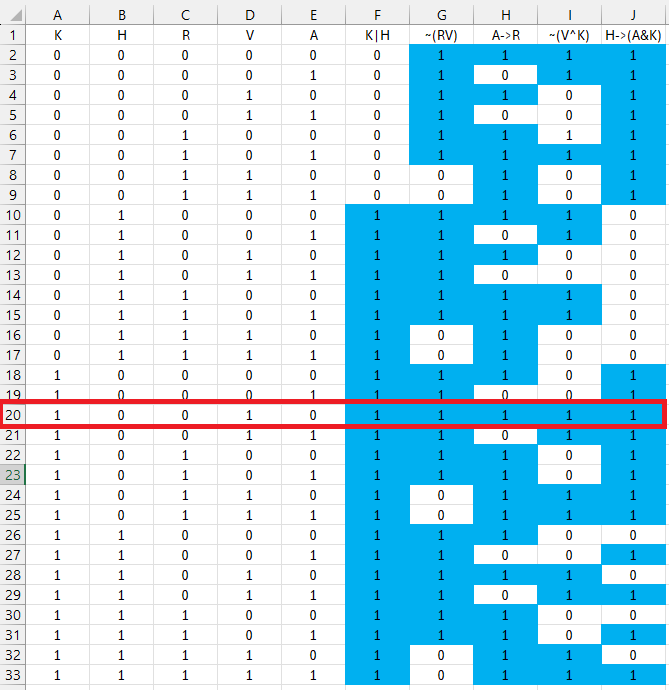
\includegraphics[scale=0.73]{p1_2-38}
    \end{figure}
    \par Lập bảng chân trị, ta thấy tập giá trị phù hợp là $(K,H,R,V,A)=(T,F,F,T,F)$. Vậy Kevin và Vijay đang chat.
\end{proof}
\subsection*{Bài 39}
Một thám tử đã phỏng vấn bốn nhân chứng của một vụ án. Qua câu chuyện của các nhân chứng, thám tử đã kết luận rằng nếu người giúp việc đang nói thật thì đầu bếp cũng nói thật; đầu bếp và người làm vườn không thể đều nói thật; người làm vườn và thợ sửa không thể đều nói dối; nếu thợ sửa nói thật thì đầu bếp nói dối. Với mỗi nhân chứng, thám tử có thể biết được rằng ai đang nói dối, ai đang nói thật hay không? Hãy giải thích.
\begin{proof}
    Đặt bốn mệnh đề, $B$, $C$, $G$, $H$ lần lượt là "Người giúp việc nói thật", "Đầu bếp nói thật", "Người làm vườn nói thật" và "Thợ sửa nói thật". \begin{itemize}
        \item Người giúp việc đang nói thật thì đầu bếp cũng nói thật: $B\rightarrow C$
        \item Đầu bếp và người làm vườn không thể đều nói thật: $\neg(C\land G)$
        \item Người làm vườn và thợ sửa không thể đều nói dối: $G\lor H$
        \item Nếu thợ sửa nói thật thì đầu bếp nói dối: $H\rightarrow\neg C$
    \end{itemize}
    Cuối cùng ta dùng phép hội với tất cả các mệnh đề, ta có: $$(B\rightarrow C)\land(\neg(C\land G))\land(G\lor H)\land(H\rightarrow\neg C)=1$$
    \begin{figure}
        \caption{Bảng chân trị bài 39, phần 1.2}
        \begin{center}
            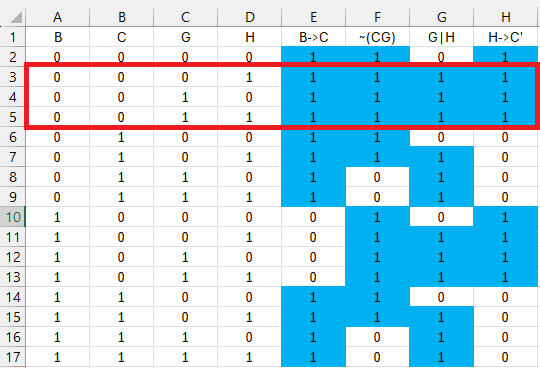
\includegraphics[scale=0.7]{p1_2-39.png}
        \end{center}
    \end{figure}
    \par Lập bảng chân trị, ta thấy có tới ba trường hợp hợp lí với giả thiết. Vì vậy thám tử chỉ biết được người giúp việc và đầu bếp nói dối, không biết được là người làm vườn và thợ sửa nói dối hay thật.
\end{proof}
\subsection*{Bài 41}
Cho rằng có các biển báo ở trên cánh cửa dẫn đến hai căn phòng. Biển báo trên căn phòng đầu tiên viết "Trong phòng này có một người phụ nữ, trong phòng kia có một con hổ"; và biển báo trên căn phòng thứ hai viết "Một trong hai căn phòng có một người phụ nữ, và trong hai căn phòng có một phòng chứa một con hổ". Cho rằng bạn biết chỉ có một biển là đúng, một biển là sai. Người phụ nữ ở đằng sau cánh cửa nào?
\begin{proof}
    Vì chỉ có một trong hai cánh cửa là thật, ta sẽ dùng phương pháp thử.
    \begin{itemize}
        \item Nếu biển báo đầu tiên đúng, nghĩa là phòng đầu có một người phụ nữ và phòng thứ hai có một con hổ. Điều này đúng với cả hai biển báo (trái ngược với giả thiết là chỉ có một biển báo đúng).
        \item Nếu biển báo thứ hai đúng, nghĩa là phòng đầu có một con hổ, phòng thứ hai có một người phụ nữ. Điều này đúng với biển báo thứ hai nhưng trái ngược với biển báo đầu tiên (hợp lí với giả thiết).
    \end{itemize}
    Vậy người phụ nữ ở sau cánh cửa căn phòng thứ hai.
\end{proof}